% Létrehozva: 2009. június 28.
\documentclass[12pt,a4paper,twoside]{article}

% Hosszú sorok helyett inkább sok hely szavak között
\sloppy

% Táblázatok formázásához
\usepackage{array}
\usepackage{multirow}

% Ábrák
\usepackage{graphicx}
\usepackage{float}

% Ékezetek, magyar nyelv
\usepackage[utf8]{inputenc}
\usepackage[T1]{fontenc}
\usepackage[hungarian]{babel}

% Forráskód megjelenítésére
\usepackage{listings}
\lstset{
  numbers=left,
  frame=shadowbox,
  numberstyle=\tiny,
  basicstyle=\ttfamily\small
}

% Definíciós lista kis whitespace-el
\newcommand{\desc}{
  \begin{description}{}{}
    \setlength\itemsep{0pt}
    \setlength\parskip{0pt}
    \setlength\topsep{0pt}
    \setlength\partopsep{0pt}
    \small}
  \newcommand{\ed}{
  \end{description}
  \normalsize }

% Elvárás a szakdolgozattal szemben a Times - sebaj
%\usepackage{times}
\fontfamily{garamond}

% Az elektronikus változatban hiperhivatkozások
\usepackage{hyperref}
% PDF tulajdonságai
\hypersetup{
  bookmarks=true,
  unicode=true,
  pdftoolbar=true,
  pdfmenubar=true,
  pdffitwindow=false,
  pdfstartview={FitH},
  pdftitle={Szakdolgozat},
  pdfauthor={Nagy Zoltán},
  pdfsubject={Online űrlapkészítő},
  pdfnewwindow=true,
  colorlinks=true
}

% Nyomtatásba
\hypersetup{
  linkcolor=black,
  citecolor=black,
  filecolor=black,
  urlcolor=black
}

% Elektronikus változat
\hypersetup{
  linkcolor=red,
  citecolor=green,
  filecolor=magenta,
  urlcolor=cyan
}

% "Oldalbeállítás"
\usepackage[margin=2.5cm, bmargin=3cm, bindingoffset=2cm]{geometry}

% Fejléc
\usepackage{extramarks}
\usepackage{fancyhdr}
\pagestyle{fancy}
\renewcommand{\sectionmark}[1]{\markright{#1}{}}
\fancyhf{}
\fancyhead[RE,LO]{\thepage}
\fancyhead[RO,LE]{\rightmark}
\fancyfoot[C]{\thepage}


\title{Szakdolgozat\\\normalsize Online űrlapkészítő}
\author{} % Kézzel helyezem el, nem oda, ahol a document classban van

\begin{document}

\maketitle\thispagestyle{empty}
\vspace{17cm}
\hspace{8cm}
Készítette: Nagy Zoltán
\clearpage

\setcounter{tocdepth}{3}
\tableofcontents

\clearpage
\phantomsection
\section{Feladatmeghatározás}

A kitűzött cél egy olyan rendszer kialakítása, amely lehetővé teszi
\texttt{HTML} űrlapok létrehozását egy point-and-click felület
segítségével. Elvárás az \texttt{HTML 4.01} szabványban meghatározott minden
\texttt{form} tagen belül legális elem támogatása. Törekedni kell a szabványos
\texttt{XHTML 1.1} kód generálására. Ezen kívül biztosítani kell
az űrlapok mentését, visszatöltését és letöltését. Opcionális cél a szerkesztés
közbeni automatikus biztonsági mentés, valamint a módosítások visszavonása.

Ennek megfelelően a projekt két jól elkülöníthető részből, illetve az ezek
közötti kommunikációból áll:
\begin{itemize}
\item A gyors válaszidő biztosítása végett a kliensoldalon kell futnia az
  űrlapszerkesztő alkalmazásnak. Ezt az alkalmazást az egyszerűség kedvéért a
  továbbiakban hívjuk \textit{Builder}nek.
\item A mentett űrlapok megtekintéséhez, módosítását és megnyitását egy
  webes felületen keresztül tesszük lehetővé. Nevezzük ezt a programrészt
  \textit{Manager}nek.
\item Biztosítani kell a Builder kapcsolatát a szerverrel az űrlap mentése és
  különböző ellenőrzések céljából.
\end{itemize}

Az alkalmazás tervezett felhasználói körébe elsősorban webmesterek
tartoznak. Nekik a majdani kód tényleges felépítése ismeretében intuitív munkafolyamatot
kell biztosítanunk. Ezen kívül az alkalmazással szemben elvárás, hogy más
szakterületű, de szintén weblapokkal dolgozó felhasználók számára is könnyen
használható legyen.

További követelmény, hogy a felhasználói felület több nyelven elérhető
legyen. Biztosítani kell a később elkészülő fordítások egyszerű hozzáadását.


\subsection{Builder}

A kliensoldali alkalmazásnak lehetőséget kell nyújtania tetszőleges elrendezés
megvalósítására. Mivel a cél egy olyan megoldás, ahol a felhasználónak nem kell
feltétlenül ismernie sem a \texttt{HTML}, sem a \texttt{CSS} leíró nyelveket,
ennek legkézenfekvőbb módja a táblázatos elrendezés. Ilyen módon megvalósítandó
a táblázat celláinak létrehozása, cellák vagy egész táblázatok törlése illetve
cellák összevonása, majd felosztása.

Az űrlapra \texttt{fieldset}ek, szöveg valamint beviteli mezők elhelyezését
kell megoldani. Az egyes elemek következő tulajdonságait kell szerkeszthetővé
tenni:

\clearpage
\desc
  \item[Táblázat cella:] Tartalom típusa (szöveg vagy beviteli mező); Szöveges
    mező esetén a szöveg, beviteli mező esetén a mező típusa és értéke/felirata
  \item[Fieldset:] Cím (\texttt{legend} elem tartalma)
  \item[Beviteli mező:] Név (\texttt{name} tulajdonság)
  \item[Select (lenyíló menü):] A kiválasztható elemek
\ed

A cella, illetve a beviteli mező típusának megváltoztatásakor célszerű elkerülni
a már beírt szöveg elvesztését. Ezért a szöveget a beviteli mező helyett a cella
tulajdonságának tekintjük, ami az egyes típusoknál a következőképpen lesz
értelmezve:

\desc
  \item[Szöveges cella:] A cella tartalma
  \item[Szöveges és jelszó beviteli mező:] Alapértelmezett érték
  \item[Radiobox, checkbox:] A box mellett megjelenítendő szöveg
  \item[Nyomógomb:] A gomb felirata
  \item[Select:] Az első opció
\ed

Lehetőséget kell adni a felhasználónak, hogy bármikor megváltoztassa a
felület nyelvét, valamint hogy a szerverre tetszőleges néven menthesse
munkáját. Ezen kívül a \texttt{HTML} kódnak bármikor megtekinthetőnek kell
lennie.

Ha szerkesztés közben megszűnne a felhasználó bejelnetkezése, lehetőséget kell
nyújtani az újbóli bejelentkezésre adatvesztés nélkül. Ha szerkesztés közben
megszűnik a szerveren az űrlap, vagy a bejelentkezett felhasználónak nincs
írásjoga az éppen szerkesztett űrlapra, mentéskor új példányt hozunk létre a
felhasználó sajátjaként.

\phantomsection
\subsection{Manager}

A mentett űrlapok kezelésére egy webes felületet fogunk
biztosítani. Bejelentkezés után a felhasználó szerkesztheti és letöltheti a
saját űrlapjait. Megjelölhet űrlapokat publikusként, amiket azután
egy kereshető listán keresztül bárki megnyithat. Más felhasználó publikus
űrlapjának mentésekor nem írjuk felül az eredetit, hanem a felhasználó
sajátjaként mentünk egy másolatot.

Ezen kívül a weblapon szerepelnie kell a szerkesztő leírásának,
kézikönyvének. Mivel az alkalmazás mindig a DOM-mal\cite{DOM} dolgozik,
\texttt{HTML} elemekkel egyszerűen megoldható az illusztráció.

A felületnek és a tartalomnak itt is több nyelven elérhetőnek kell lennie.

\clearpage
\phantomsection
\section{Környezet}

\paragraph{Webszerver}
A fejlesztés és tesztelés \textbf{Apache 2.2.11} szerveren történt. Az
alkalmazás felhasználóbarát URL-eket hoz létre, ezért módosítás nélkül nem
használható olyan környezetben, ahol a \texttt{mod\_rewrite} (vagy vele
egyenértékű modul) nem elérhető.

\paragraph{PHP értelmező}
A Manager PHP programnyelven íródott, így mindenképpen PHP értelmező futtatására
képes webszerverre van szükség. Gyorsabb fejlesztés, jobb karbantarthatóság és
logikusabb felépítés elérése végett a \textbf{CodeIgniter}\cite{CI} framework
\textbf{1.7.1}-es verzióját használtam. A frameworknek 4.3.2-es verziójú
PHP értelmezőre van szüksége, de az alkalmazás működéséhez minimum \textbf{PHP
  5.2.0} kell. A \texttt{php.ini}-ben engedélyezni kell a json, mysql
és session kiegészítéseket.

\paragraph{Adatbázis szerver}
Az adatbáziskezelés csak \textbf{MySQL 5.1.37} adatbázison volt tesztelve, de a
CI ActiveRecord\cite{CI-ActiveRecord} szolgáltatás használata miatt az
alkalmazás módosítás nélkül működik az CI által támogatott SQL
szervereken\cite{CI-Req}. Az adatbázis-szerver típusát és a kapcsolódáshoz
szükséges adatokat a \texttt{system/application/config/database.php} fájlban
kell beállítani, legalább az alábbi sorok szerkesztésével:

\begin{lstlisting}[language=PHP, firstnumber=40]
$db['default']['hostname'] = "db_host";
$db['default']['username'] = "username";
$db['default']['password'] = "password";
$db['default']['database'] = "db_name";
$db['default']['dbdriver'] = "mysql";
// TODO kivenni: $ (hogy LaTeX hilight boldog legyen)
\end{lstlisting}

\paragraph{JavaScript}
A Builder JavaScript programnyelven íródott a \textbf{jQuery}\cite{JQ} library
\textbf{1.3.2} verziójával. A dinamikusan létrehozott DOM elemek egyszerű
kezelésére a \textbf{LiveQuery}\cite{JQ-LiveQuery} plugin \textbf{1.0.3}
verzióját használja. Ezeken kívül mind a Builder, mind a Manager használja
kis részben a \textbf{jQuery-UI}\cite{JQ-UI} Draggable, Dialog és Tabs
komponenseit. A felhasználó letöltési idejének minimalizálása érdekében a
JavaScript és CSS fájlok méretét a \textbf{YUI Compressor}\cite{YUI} segítségével
csökkentettem.

\paragraph{Böngészők}
Az alkalmazást a Firefox (és más XULRunner alapú) és az Opera böngészőkkel
teszteltem. Jelenlegi állapotában az Internet Explorer böngészők JavaScript
értelmezőjével a Builder nem működik.

\paragraph{Szakdolgozat}
Jelen dokumentum a \textbf{LaTeX} rendszer TexLive disztribúcióból származó
3.1415926 verziójával készült az \textbf{Emacs} szerkesztőben, az
\textbf{AUCTeX} csomag segítségével. A diagrammok létrehozására a \textbf{Dia 0.97}
szerkesztőt használtam.


\clearpage
\phantomsection
\section{Adatbáziskezelés}

A karbantartás könnyítése és az átláthatóság megőrzése érdekében mindenképpen
célszerű az adatbázis kezelését végző kódot elkülöníteni a felhasználói
felülettől és a felhasználói bemenet kezelésétől. Erre egy bevett módszer az
MVC\cite{MVC} minta implementálása, amit a CodeIgniter framework jelen esetben
elvégez helyettünk. Ilyen módon az adatbázis-kezelés néhány modell megírásából
áll. Az adatbázis-szerkezet leírása után a modellek által létrehozott
absztrakciós szint ismertetése következik.

\phantomsection
\subsection{Adatbázis-szerkezet}

Az alkalmazás szempontjából kritikus adatok a felhasználó azonossága, a hozzájuk
tartozó űrlapok és az egyes űrlapok tartalma. Ezek köré szerveződik az egyszerű
szerkezet: a felhasználók és az űrlapok számára létrehozunk két táblát, közöttük
pedig $1..n$ kapcsolatot állítunk fel. A kapcsolómező a felhasználó
azonosítója. Ezen a szinten feleslegesnek tűnik a az űrlapokat külön
azonosítóval ellátni, de lehetőséget akarunk biztosítani az űrlapok
átnevezésére; emiatt az űrlapok egyedi azonosítására ez a legegyszerűbb módszer.

Az ábrán és a táblázatokban megadott adattípusok a MySQL adatbázis típusai.

% Adatbázis diagramm
\begin{figure}[htp]
  \centering
  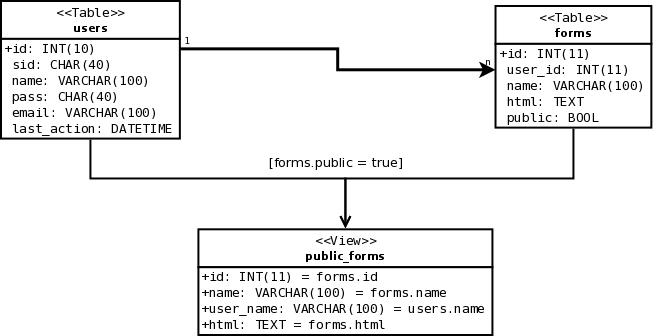
\includegraphics[width=328px]{db.png}
  \caption{Adatbázis-szerkezet}\label{fig:db}
\end{figure}

% users tábla
\subsubsection{\texttt{users} tábla}
A \texttt{sid} és \texttt{last\_action} mezőket a felhasználók bejelnetkezésének
ellenőrzésekor használjuk (TODO: lásd itt-és-itt)

\small
\vspace{.3cm}
\begin{tabular*}{\textwidth}{>{\tt}l>{\tt}l>{\tt}l>{\tt}l|l}
  \rm Név       &  \rm Típus  &  \rm Méret  & \rm Index/Kulcs & Megjegyzés           \\
  \hline
  id           &   INTEGER AUTO\_INCREMENT && PRIMARY KEY    &                      \\
  sid          &   CHAR      & 40          &                 &  PHP session cookie  \\
  name         &   VARCHAR   & 30          & INDEX           &                      \\
  pass         &   CHAR      & 30          &                 &  SHA1 hash (hex)     \\
  email        &   VARCHAR   & 100         & INDEX           &  Nem nyilvános       \\
  last\_action &   DATETIME  &             &                 &
\end{tabular*}
\normalsize

% forms tábla
\subsubsection{\texttt{forms} tábla}

A \texttt{user\_id} mezővel kapcsoljuk az űrlapot a létrehozó felhasználóhoz. A
\texttt{html} mező tárolja magát az űrlapot (a \texttt{<form>} elem nélkül), míg
a \texttt{public} mező adja meg, hogy az űrlap megjelenhet-e a nyilvános űrlapok
listáján.

\small
\vspace{.3cm}
\begin{tabular*}{\textwidth}{>{\tt}l>{\tt}l>{\tt}l>{\tt}l|l}
  \rm Név    & \rm Típus &  \rm Méret  & \rm Index/Kulcs & Megjegyzés\\
  \hline
  id        & INTEGER AUTO\_INCREMENT && PRIMARY\_KEY   &                            \\
  user\_id  & INTEGER   & 11          & INDEX           & $1..n \rightarrow{}$ users \\
  html      & TEXT      &             &                 &                            \\
  public    & BOOL      &             & INDEX           &
\end{tabular*}
\normalsize

% public_forms nézet
\subsubsection{\texttt{public\_forms} nézet}

Az adatbázis szerkezetének szempontjából lényegtelen, de megkönnyíti a nyilvános
űrlapok kiválasztását, és lehetőséget ad az adatbázismotornak az
optimalizálásra. A nyilvános űrlapokat listázza azonosítójukkal, nevükkel, a
létrehozó felhasználó nevével és az űrlap tartalmával.

A MySQL adatbázis-rendszer támogatja az írható nézeteket, de számos más rendszer
nem, így ezt a nézetet csak olvasásra használjuk.

\small
\vspace{.3cm}
\begin{tabular*}{\textwidth}{>{\tt}l>{\tt}l>{\tt}l|>{\tt}l}
  \rm Név     &  \rm Típus    &  \rm Méret  & Megjegyzés \\
  \hline
  id         &  INTEGER      &  11         & forms.id   \\
  name       &  VARCHAR      &  100        & forms.name \\
  user\_name &  VARCHAR      &  100        & users.name \\
  html       &  TEXT         &             & forms.html
\end{tabular*}
\normalsize
% ----- Adatbázis-szerkezet vége -----


\phantomsection
\subsection{Modellek}

A CodeIgniter a modelleket a \texttt{system/application/models} mappában
tárolja. Az alkalmazás két modellt használ: egyet a felhasználók kezelésére
(\texttt{user\_model}) és egyet az űrlapok kezelésére (\texttt{forms\_model}). A
\texttt{user\_model} csak a \texttt{users} táblát, míg a
\texttt{forms\_model} szükségszerűen mindkét táblát és a \texttt{public\_forms}
nézetet is használja.

A lekérdezések összeállításához és futtatásához a CodeIgniter ActiveRecord
szolgáltatását használjuk. Ezzel egy tipikus lekérdezés a következőképpen
valósul meg:

\begin{lstlisting}[language=PHP]
function get_form_public($id)
{
  // WHERE feltetel asszociativ tombben
  $where = array('id' => $id);

  // Lekerdezes es eredmeny
  $this->db->from('public_forms')->where($where);
  $result = $this->db->order_by('id')->get();

  // Nincs ilyen azonositoju publikus urlap
  if ($result->num_rows() == 0)
  return false;

  $row = $result->row();

  $user = $this->user->get_user(false);

  // Ha van bejelentkezett felhasznalo...
  if ($user !== false)
  // Es az ove az urlap, tudatjuk a hivoval
  $row->owner = ($user->name == $row->user_name);

  // Visszaadjuk az eredmenyt
  return $row;
  // TODO kivenni: $ (hogy LaTeX hilight boldog legyen)
}
\end{lstlisting}

\phantomsection
\subsubsection{\texttt{user\_model}}

\paragraph{Regisztráció}
Itt történik a felhasználók regisztrálásához valamint ki- és bejelentkezéséhez
szükséges adatbáziskezelés. Új felhasználó regisztrációjakor ellenőrizni
kell, hogy a megadott felhasználónév és e-mail szerepel-e a már az
adatbázisban. Az e-mail ellenőrzését a \texttt{check\_email}, a felhasználónév
ellenőrzését pedig a nem túl szerencsés nevű \texttt{not\_available} függvény
végzi. A \texttt{register} függvény csak akkor kerül meghívásra, ha már
meggyőződtünk a kapott adatok helyességéről (TODO: lásd login\_controller kapott
adatok ellenőrzése).

TODO:
Az e-mail címet jelenleg nem használjuk fel, de később a regisztrációról történő
értesítésre lehet használni.

A \texttt{get\_user} függvény a bejelentkezett felhasználó adatait, vagy ennek
hiányában a \texttt{false} értéket adja vissza. Ha van bejelnetkezettt
felhasználó, akkor itt futtatjuk az \texttt{update\_last\_action} függvényt,
ezzel biztosítva, hogy minden műveletnél frissítjük a felhasználó
bejelentkezését.

\paragraph{Bejelentkezés}
Igaz ugyan, hogy ennél az alkalmazásnál a biztonság nem elsődleges szempont, de
így is szükség van a felhasználók bizonyos szintű védelmére. A jelszavakat és
a bejelentkezett felhasználó PHP-től kapott munkamenet-azonosítóját (session
id\cite{PHP-SID}) egyirányű titkosítás után tároljuk - előbbit a
\texttt{users.pass}, utóbbit a \texttt{users.sid} mezőben.

A felhasználónév és jelszó ellenőrzése a \texttt{login} függvényben
történik. Sikeres bejelentkezés esetén, tehát ha a megadott név/jelszó páros
szerepel az adatbázisban, az adott rekordba eltároljuk az aktuális munkamenet
azonosítóját (titkosítás után). A bejelentkezés sikerességérők a visszatérési
értékkel értesítjük a hívót.

A modellben elvárjuk az alkalmazás többi részétől, hogy minden művelet
elvégzésekor meghívja az \texttt{update\_last\_action} függvényt. Ezzel az
aktuális munkamenethez tartozó \texttt{users.last\_action} mező értékét a
jelenlegi időpontra állítjuk. Sikeres bejelentkezéskor is frissítjuk a dátumot.

\paragraph{Kijelentkeztetés}
A felhasználót csak akkor tekintjük bejelentkezettnek, ha a
munkamenet azonosítója szerepel az adatbázisban, és a hozzá tartozó utolsó
művelet nem régebbi egy napnál. A felhasználó kézi kijelentkezése esetén a
\texttt{logout} függvényben munkamenet-azonosítót töröljük (üres sztringre állítjuk).


\phantomsection
\subsubsection{\texttt{forms\_model}}

Az űrlapok létrehozását, mentését, törlését, átnevezését és listázását kezelő
függvények. Az olvasás jellegű műveletek visszatérési értéke vagy a lekérdezés
eredménye, vagy (eredménytelen lekérdezés esetén) \texttt{false}. Az írás
jellegű műveletek eredménye mindig \texttt{true} vagy \texttt{false}.

Másik szempontból csoportosítva beszélhetünk nyilvános és privát műveletekről. A
privát műveletek csak bejelentkezett felhasználók számára elérhetőek - a
felhasználói felület szintjén is, de ha eljut egy hívás a modellig,
a futás bejelentkezett felhasználó hiányában hibával megáll. Két kivétellel az
összes függvény privát: a \texttt{get\_form\_list\_public} és a
\texttt{get\_form\_public} függvények csak publikus űrlapokkal dolgoznak. Itt
használjuk ki a \texttt{public\_forms} nézetet.


\phantomsection
\section{Manager}

A webes felület a modellek, vezérlők (controller), nézetek (view) és nyelvi fájlok
együttműködéséből áll össze. Ezért egy-egy fájl helyett több fájl bizonyos
részei alkotnak logikai egységet. Az egységek általában a felhasználó által
végezhető művelet vagy műveletek kezelését és az eredmény megjelenítését foglalják
magukban. Ezeken a művelet-központú egységeken kívül bemutatásra kerül a
felhasználóbarát URL-ek használhatóvá tevő rendszer, a vezérlők alaposztálya
és az új fordítások hozzáadásának módja is. Sok függvény elfogad egy opcionális
\texttt{\$lang} paramétert, aminek az alapértelmezett értéke \texttt{null}. Ez a
felhasználói felület kívánt nyelvét jelöli.


\phantomsection
\subsection{Routing - felhasználóbarát URL-ek}

A CodeIgniter framework routing\cite{CI-Routing} szolgáltatásán keresztül
könnyen használhatunk felhasználók számára is könnyen olvasható URL-eket.
A framework a futtatandó függvényt a következő módon olvassa ki az oldal
címéből: \texttt{példa.com/vezérlő/függvény/paraméter1/paraméter2}.
A \texttt{system/application/config/routes.php} fájlban megadhatunk más,
tetszőleges címeket, amiket aztán az előbbi formátumú URI-khez rendelünk. Az
URL-ek megadásánál használhatunk reguláris kifejezéseket\cite{regex}, így szinte
bármilyen helyzetnek megfelelő szabályokat fel tudunk állítani. A használt
beállítások:

\begin{lstlisting}[language=PHP, firstnumber=46]
$langs = '(en|hu)';

$route[$langs]           = 'home/index/$1';
$route['(:any)/'.$langs] = '$1/index/$2';
$route['logout']         = 'login/logout';
$route['builder/(:num)'] = 'builder/open/$1';
// TODO kivenni: $ (hogy LaTeX hilight boldog legyen)
\end{lstlisting}

A 46. sorban egy reguláris kifejezés segítségével megadjuk azokat a
nyelv-azonosítókat, amik szerepelhetnek érvényes címekben. Ezeknek az
azonosítóknak meg kell egyezniük a nyelvi fájlokban használt azonosítókkal
(TODO: lásd fordítások hozzáadása).

Az alábbi táblázatban az átirányítási szabályokra szerepel egy-egy példa. A
``pelda.com'' a \texttt{system/application/config/config.php} fájlban megadott
\texttt{base\_path} érték.

\begin{tabular*}{\textwidth}{>{\tt}l|>{\tt}r>{$\rightarrow$}c>{\tt}l}
  \rm Sor & \rm Honnan           & & \rm Hova        \\
  \hline
  48      & pelda.com/hu         & & pelda.com/home/index/hu  \\
  49      & pelda.com/teszt/hu   & & pelda.com/teszt/index/hu \\
  50      & pelda.com/logout     & & pelda.com/login/logout   \\
  51      & pelda.com/builder/20 & & pelda.com/builder/open/20
\end{tabular*}


\phantomsection
\subsection{BaseController - a vezérlők alaposztálya}

A \texttt{system/application/controllers/BaseController.php} fájlban található
osztályban összegyűjtöttem azokat a függvényeket és beállításokat, amikre
bármelyik vezérlőben szükség lehet.

\paragraph{\texttt{render(\$return=false)}}
Mivel a Buildert alkalmazáson kívül minden oldalon megtalálhatóak bizonyos
elemek - a fejléc, a menü, a lábléc - logikus lépés volt ezeknek az állandó
elemeknek egy nézetbe foglalása. A CodeIgniter lehetőséget ad rá, hogy a
nézetet betöltő függvénynek átadjunk egy tömböt, aminek a tartalma elérhető lesz
a nézetből - a kulcsok lesznek a változók nevei, az értékek pedig értelemszerűen
a tömb értékei.

Az állandó elemeket tartalmazó \texttt{skeleton} nézetnek a vezérlő
\texttt{slots} nevű tulajdonságát adjuk át. Így a megjelenítendő elemeket a
vezérlő futása során bármikor módosíthatjuk. Az aktuális oldal tartalmát a
\texttt{slots} tulajdonság \texttt{content} kulcsához rendeljük. Ez általában
egy másik nézet futtatásának eredménye, amit nem megjelenítettünk, hanem egy
változóban tároltunk. A \texttt{render} függvény \texttt{\$return} paramétere is
ezt a célt szolgálja - ha értéke \texttt{true}, akkor az eredményt megjelenítés
helyett visszaadjuk a hívó függvénynek.

Még a tényleges megjelenítés előtt felépítjük a menüt a \texttt{builde\_menu}
függvény és a \texttt{menu} nézet segítségével, majd ha van a vezérlő nevével
megegyező fájlnevű javascript, illetve css fájl, ezeket is átadjuk a
\texttt{skeleton} nézetnek.

\paragraph{\texttt{check\_login(\$redirect='my\_forms')}}
Ez a függvény ellenőrzi, hogy van-e bejelentkezett felhasználó, és ha nincs,
akkor átirányítja a felhasználót a bejelentkező olralra. Onnan sikeres
bejelentkezés vagy regisztráció után a \texttt{\$redirect} paraméterben tárolt
oldalra fog kerülni.

\paragraph{\texttt{remote\_check\_rights}}

Ezt a függvényt AJAJ kérésekkel hívjuk a felhasználó jogainak ellenőrzése
céljából. A POST adatokból a \texttt{write} és az \texttt{id} paramétereket
olvassa be. A \texttt{write} a végzendő művelet típusára utal - ha
\texttt{true}, akkor írni, ha \texttt{false}, akkor olvasni akarunk.
Az \texttt{id} paraméter a módosítani vagy olvasni kívánt űrlap azonosítója.
A lehetséges eredmények:

\desc
  \item[OK:] A felhasználónak van joga a megadott művelethez
  \item[NOT\_LOGGED\_IN:] A kért művelethez bejelentkezett felhasználóra van szükség
  \item[FORM\_NOT\_FOUND:] A felhasználónak nincs joga kért művelethez, vagy az űrlap
    nem található.
\ed

Az eredmény kiválasztásának folyamatát a következő ábra mutatja be.

\begin{figure}[h]
  \centering
  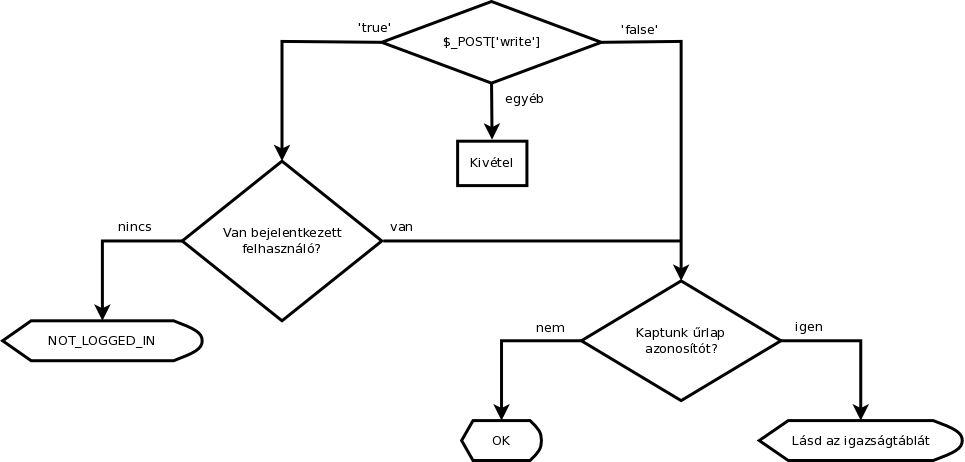
\includegraphics[width=400px]{rights.png}

  \desc\small
    \item[WRITE:] A POST-ban kapott \texttt{write} paraméter
    \item[PRIV:] Az űrlap az éppen bejelentkezett felhasználóhoz tartozik?
    \item[PUB:] Az űrlap publikus?
  \ed\normalsize

  \begin{tabular*}{\textwidth}{r|cc|cc}
    \multirow{2}{*}{WRITE} & \multicolumn{2}{c|}{PRIV = 1} & \multicolumn{2}{c}{PRIV = 0} \\
    & PUB = 1 & PUB = 0 & PUB = 1 & PUB = 0 \\
    \hline
    true  & OK & OK & NOT\_FOUND & NOT\_FOUND \\
    false & OK & OK & OK         & NOT\_FOUND \\
  \end{tabular*}

  \caption{Felhasználói jogok ellenőrzése}\label{fig:rights}
\end{figure}


\paragraph{\texttt{load\_lang(\$file, \$in=null)}}
Betölti a kért nyelvi fájlt a megfelelő nyelvi fájlból. Az \texttt{\$in}
paraméter a vezérlőkben megjelenő \texttt{\$lang} opcionális paraméter értékét
kapja. Ha tehát az URL-ben szerepel egy nyelv, akkor itt töltjük be az annak
megfelelő sztringeket. Ezen kívül elmentjük a munkamenetbe a nyelvet, amit akkor
használunk, ha az URL-ből nem kaptunk nyelvet. Ha még a munkamenetben sincs
mentett nyelv, akkor a konstruktorban megadott első nyelvet használjuk.


\phantomsection
\subsection{Új fordítások hozzáadása}

A felhasználói felület nyelvi fájljait a Manager és a Builder külön tárolja: a
Manager a \texttt{system/application/language} mappában, a Builder pedig a
\texttt{scripts/builder/translations.js} fájlban. Egy új nyelv hozzáadása négy
lépésből áll:

\begin{itemize}
  \item A nyelv azonosítójának kiválasztása. Általában a legegyszerűbb az
    \texttt{img/famfamfam/png} mappában található zászló nevével megegyező
    azonosítót választani. Ez a spanyol nyelv esetén például
    \texttt{es}. Ellenkező esetben a zászlóról készíteni kell egy
    másolatot, aminek a neve megegyezik az azonosítóval, hiszen a nyelvek
    kiválasztását lehetővé tevő menü ezt a képet fogja használni.
  \item A Manager felületének lefordítása. Egy már létező fordítás fájljait
    (például a \texttt{system/application/language/hu} mappa tartalmát)
    lemásoljuk az új nyelv azonosítójával megegyező nevű mappába, majd
    elvégezzük a fordítást.
  \item A \texttt{BaseController} osztály konstruktorában a
    \texttt{\$this->lang\_names} tömbhöz hozzáadjuk az új nyelv azonosítóját és
    nevét. Például az angol, magyar és spanyol nyelvekkel a tömb a következő
    értéket kapná:
    \begin{lstlisting}[firstnumber=35]
$this->lang_names = array('en' => 'English',
                          'hu' => 'Magyar',
                          'es' => 'Espanol'
                         );
// TODO kivenni: $ (hogy LaTeX hilight boldog legyen)
    \end{lstlisting}
    Így az új nyelv be fog kerülni a nyelv kiválasztását lehetővé tevő menübe.
  \item A \texttt{system/application/config/routes.php} fájlban a
    \texttt{\$langs} változóhoz hozzáadjuk a nyelv azonosítóját. Például az
    angol, magyar és spanyol nyelvekkel a változó a következő értéket kapná:
    \begin{lstlisting}[firstnumber=46]
$langs = '(en|hu|es)';
// TODO kivenni: $ (hogy LaTeX hilight boldog legyen)
    \end{lstlisting}
    Így a \texttt{*/es} alakú oldalak megnyitásakor ``Az oldal nem található''
    hiba helyett spanyol nyelven nyílik meg a kért oldal.

\end{itemize}

Ezen kívül még le kell fordítani a Builder felületének üzeneteit is - ezt a
(TODO: lásd ott) részben tárgyalom.

\phantomsection
\subsection{Regisztráció}

A tényleges regisztrációt a \texttt{users\_model} hajtja végre. A feladatunk itt
a felhasználó által megadott adatok ellenőrzése. Ellenőrizni
kell a megadott felhasználónév és e-mail cím létezését. Figyelni kell az e-mail
cím helyességére, a két jelszó mező egyezésére, valamint a kapott adatok
hosszára - egy megadott minimum hossz és az adatbázisban meghatározott
maximális hosszúság közé kell esnie.

Az adatok ellenőrzésére, illetve ezekről visszajelzés küldésére négy
lehetőségünk van:

\paragraph{Csak szerveroldali ellenőrzés}
Az űrlap kitöltése után közvetlenül a szervernek küldjük az adatokat, majd egy
újragenerált lapon értesítjük a felhasználót a regisztráció sikerességéről, vagy
a hibaüzenetekről. Utóbbi esetben a kapott adatokkal feltöltve adjuk vissza az
űrlapot. Ennek a megoldásnak a megvalósítását jelentősen megkönnyíti a
CodeIgniter framework Validation osztálya\cite{CI-Val}. A felhasználónak meg kell várnia az új lap
letöltését és kitöltés közben nem kap visszajelzést a megadott adatok
helyességéről.

\paragraph{Csak kliensoldali ellenőrzés}
A felhasználó szempontjából kényelmes, hiszen azonnali visszajelzést kap a
megadott adatokról, ráadásul a lap újratöltésére sem kell várnia hiba
esetén. Biztonsági szempontból azonban elfogadhatatlan megoldás, hiszen egy
esetleges támadónak elég egy hibás kérést küldenie a szervernek. Ráadásul a
kliensoldali ellenőrzés visszajelzéseiből megtudja, hogy milyen adatokkal tud
hibát okozni.

\paragraph{Önálló ellenőrzés a szerveren és a kliensen}
A fenti módszerek előnyeit egyesíti, hátrányaikat kiküszöböli. A kliensoldali
ellenőrzés miatt a felhasználó számára kényelmes, a szerveroldali ellenőrzés
miatt biztonságos. Könnyű kezelni azt az esetet is, ha a kliens nem tudja
futtatni az ellenőrzést (pl. a böngészőben le van tiltva a JavaScript
futtatása). Hátrány, hogy minden ellenőrzést implementálni kell mind
a szerveren, mind a kliensoldali nyelven. Így felesleges redundanciát vezettünk
be - az ellenőrzési kritériumok változásait két helyen kell módosítani, kétszer
kell tesztelni.

Ez a fajta probléma elkerülhető némi metaprogramozás bevezetésével, például a
CodeIgniter által használt kritérium-leírásokhoz hasonló nyelvvel
\cite{CI-Val}. Ha a szerveren és a kliensen futó ellenőrzés is ugyanazt a
szabályleíró fájlt használja, akkor elkerültük az ellenőrzendő esetek
ismétlését. A redundancia így átkerül a szabályleírást értelmező programrészbe,
ami valószínűleg bonyolultabb, mint maguk az ellenőrzések. Nagy számú
ellenőrzésnél ez jó megoldás lehet, de ennél az alkalmazásnál túlzás.

\paragraph{Szerveroldali ellenőrzés és AJAJ}
AJAJ-nak az AJAX (Asynchronous JavaScript and XML \cite{ajax}) technológia egy
olyan változatát nevezzük, ahol az adatok továbbítása XML helyett JSON
(JavaScript Object Notation \cite{json}) formátumban történik. Így kisebb
sávszélességet használunk, és a kliensoldalon az adatok feldolgozása egyszerűbbé
válik (bár a jQuery library képes XML-ből is JavaScript objektumokká alakítani a
kapott adatokat).

A tényleges ellenőrzést ennél a megoldásnál a szerveren végezzük, és lehetővé
tesszük, hogy a felhasználói felület szerkesztés közben a szervert megkérje
egyes adatok ellenőrzésére. Így az előző megoldás redundanciáját kiküszöböltük
néhány bájt hálózat-forgalom ellenében. A szerver terhelése így valamivel nő, de
ennél az alkalmazásnál méreténél fogva valószínűsíthető, hogy nem fognak
skálázhatósági problémák fellépni.

Kérdés viszont, hogy az űrlap elküldését hogyan valósítsuk meg.
A kliensoldali ellenőrzések aszinkron volta miatt a legegyszerűbb módszer, az
űrlap \texttt{onsubmit} eseményének használata nem megoldható: itt visszatérési
értékre van szükség, amit átlagos AJAJ hívásnál nem kapunk. Az eredmények
összegyűjtése utáni küldés nem megoldás, hiszen előfordulhat, hogy közben a
felhasználó még módosít az űrlapon. Lehetőség van szinkron, blokkoló módon
futtatni az ellenőrzéseket, de a mai böngészőkben ilyenkor a felhasználó a kérés
teljesítéséig semmit sem tud tenni.

Ezt a problémát a csak szerveroldali ellenőrzésnél hátrányként említett módon
oldottam meg: hiba esetén a regisztrációs oldal újra letöltődik. Mivel a
beviteli mezők szerkesztésekor az \texttt{onchange} eseményre induló ellenőrzés
jelzi a felhasználónak a megadott adatok helyességét, ez ritkán fog előfordulni.

\phantomsection
\subsubsection{Szerveroldal}

% Registration check folyamatábra
\begin{figure}[htp]
  \centering
  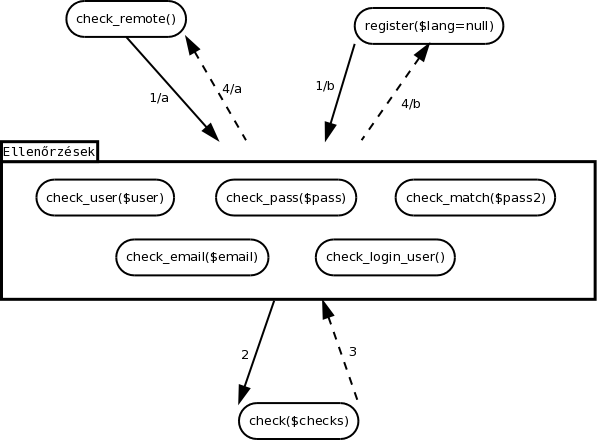
\includegraphics[width=328px]{reg_check.png}
  \caption{Regisztrációs adatok ellenőrzése}\label{fig:reg_check}
\end{figure}

Az regisztrációnál megadott adatok ellenőrzése két helyről indulhat. Ha a kliens
kérte az ellenőrzést, akkor a \texttt{check\_remote} függvényen keresztül hívjuk
meg a kért ellenőrzést (\emph{1/a}). Ha a felhasználó már elküldte az űrlapot,
akkor a \texttt{register} függvény lefuttatja az összes ellenőrzést
(\emph{1/b}). Az \texttt{Ellenőrzések} a kapott adatok biztonságossá tétele után a
\texttt{check} függvényen keresztül végzik el az adatok tényleges ellenőrzését
(\emph{2, 3}), majd visszaadják az eredményt a hívó függvénynek (\emph{4/a, 4/b}).


\paragraph{\texttt{check(\$checks)}}
Ez a függvény megkönnyíti az ellenőrzések elvégzését, a hozzájuk szükséges kódot
lerövidíti. A \texttt{check\_*} függvények előkészítik számára az ellenőrzéseket
egy-egy sztring formájában, ami a futtatandó ellenőrzést tartalmazza PHP kód
formájában. Ezekben az ellenőrző kódokban a vezérlőt (controller) a
\texttt{\$controller} változón keresztül lehet elérni. Erre például a
felhasználónév létezésének ellenőrzésénél van szükség.

A kapott paraméter egy asszociatív tömb, ahol a kulcs a futtatandó ellenőrzés,
az érték pedig egy vektor: a hiba esetén megjelenítendó üzenet azonosítója és
az abba behelyettesítendő értékek. Az üzenet tényleges szövegét az aktuális
nyelvnek megfelelő nyelvi fájlból fogjuk kiolvasni. A behelyettesítendő érték
lehet például nem megfelelő hosszúságú adatnál a minimális vagy maximális
megengedett hosszúság.

A ténylegesen futtatott
ellenőrző-függvényt a \texttt{create\_function} függvénnyel hozzuk létre. Ha
például a kapott ellenőrző kód:
\texttt{"\$controller->user->not\_available('foo')"}, akkor a létrehozott
függvény a következő:

\begin{lstlisting}[language=PHP, numbers=none]
function lambda($controller)
{
  return ($controller->user->not_available('foo'));
}
\end{lstlisting}

A függvénynek a \texttt{\$controller} paraméterbe a \texttt{\$this} értékét
adjuk át, ezzel biztosítva a hívó vezérlő elérhetőségét az ellenőrzésen
belül. Ha az így létrehozott és futtatott függvény visszatérési értéke
\texttt{false}, akkor az ellenőrzéshez tartozó üzenetleíró vektort hozzáadjuk a
hibák listájához, amit aztán az összes ellenőrzés lefuttatása után visszaadunk a
hívó függvénynek.


\paragraph{\texttt{Ellenőrzések}}
Az \texttt{check\_} prefixumú függvények egyetlen paraméterükként az
ellenőrzendő értéket várják. Még a \texttt{check\_pass\_match} függvény is, ami
a megadott jelszavak ellenőrzését végzi - itt az egyik jelszót a POST adatokból
olvassuk ki. Mivel az ellenőrzendő és a hiba esetén újra kitöltendő mezők neve
ugyanazon tömbben szerepel, és a bejelnetkezési űrlap nevét nem ellenőrizzük
változtatásakor, a \texttt{check\_login\_user} függvény mindig egy üres tömböt
ad vissza - ezzel jelezve, hogy nincsenek hibák.

Az adott ellenőrzésekre jellemző adatok (például minimum és maximum hosszúság)
beállítása után a vizsgálni kívánt adatokban a \texttt{'} karaktereket
\texttt{\textbackslash'}-re cseréljük, mivel az ellenőrzéseket először sztringekként állítjuk
össze. A cserével kivédjük a SQL injectionhöz hasonló támadásokat.

Végül a szükséges ellenőrzéseket és hozzájuk tartozó hibaüzeneteket átadjuk a
\texttt{check} függvénynek, aminek az eredményét feldolgozás nélkül visszaadjuk
a hívónak. Itt nem dolgozzuk fel a hibaüzeneteket, hiszen nem tudhatjuk, hogy a
hívó függvény hogyan kívánja értesíteni a felhasználót, vagy az őt hívó
függvényt.


\paragraph{\texttt{check\_remote}}
Ezt a függvényt érik el a kliens ellenőrzési kérései egy POST hívás
segítségével. Egy hívás pontosan egy mező ellenőrzését kéri, tehát pontosan egy
\texttt{check\_*} függvény futását fogja eredményezni. Ha visszakapott, hibákat
tartalmazó tömb üres, akkor a \texttt{true} sztringet írjuk ki, ami JSON-ként
való értelmezés után a \texttt{true} bináris értéket fogja képviselni a
kliensoldalon.

Ha vannak hibák, akkor a hozzájuk tartozó üzenetet adjuk vissza idézőjelek
között - így a JSON értelmezése után a kliensoldalon is sztringet kapunk. Ha
több hiba van, akkor is csak az elsőt adjuk vissza. Ha például egy kötelezően
kitöltendő mező üres, akkor elég csak a ``Kitöltés kötelező'' üzenetet kiírni, a
``Legalább 5 karakter hosszú legyen'' figyelmeztetés felesleges.


\paragraph{\texttt{register(\$lang=null)}}
Ez a függvény kezeli az elküldött regisztrációs űrlapot. Lefuttatja az összes
ellenőrzést, és ha bármelyik hibával tér vissza, visszaküldi a felhasználót a
regisztrációs oldalra a felhasználónév és e-mail mezők értékét feltöltve a
felhasználó által megadottakkal.

Ha nincs hiba, \texttt{user\_model} \texttt{register} függvényén keresztül
elvégzi az ellenőrzést, és a POST adatok között kapott \texttt{redirect} oldalra
irányítja a felhasználót.


\subsubsection{Kliensoldal}

A kliens feladata csupán annyi, hogy szerkesztéskor, illetve hibás űrlap küldése
után elvégeztesse a szerverrel a megfelelő ellenőrzéseket, és megjelenítse az
eredményt a felhasználó számára.

Az ellenőrzés meghívását és az eredmény kezelését a \texttt{check\_ajaj}
függvény végzi. A jQuery framework segítségével elküldi a \texttt{data}
paramétert a fenti \texttt{check\_remote} függvénynek, majd az eredménynek
megfelelő képet és üzenetet helyez el az \texttt{\$input} paraméterben kapott
beviteli mező után. A Builderben is megjelenő \$ prefixumú változónevek arra
utalnak, hogy a tárolt érték egy jQuery objektum. Ha a \texttt{check\_ajaj}
függvény \texttt{initial} paramétere \texttt{true}, akkor az üres mezőknél is
megjelenítjük a hibaüzeneteket. Ez csak közvetlenül az oldal betöltődése után
fordul elő, és az üresen elküldött mezők jelölésére szolgál.

A \texttt{check} függvény a \texttt{name} paraméterben átadott mező értékének
ellenőrzésére szolgál. Eltávolítja az előző ellenőrzések eredményeit az
űrlapról, majd a mező értékéből és a \texttt{name} paraméterből összeállított
\texttt{data} paraméterrel meghívja a \texttt{check\_ajaj} függvényt. Az
\texttt{\$input} paraméterbe értelemszerűen az ellenőrzött beviteli mező kerül,
az \texttt{initial} értéket pedig egyszerűen továbbadja. A
\texttt{check\_pass\_match} függvény hasonló módon működik, de \texttt{data}
értékeit a szerveroldali \texttt{check\_pass\_match} függvénynek megfelelő
formában állítja össze.

Mindkét függvényt a beviteli mezők \texttt{onchange} eseményének futásakor és az
oldal betöltődésekor hívjuk meg.


\clearpage
\phantomsection
\subsection{Saját űrlapok listázása}

\centering
\begin{figure}[H]
  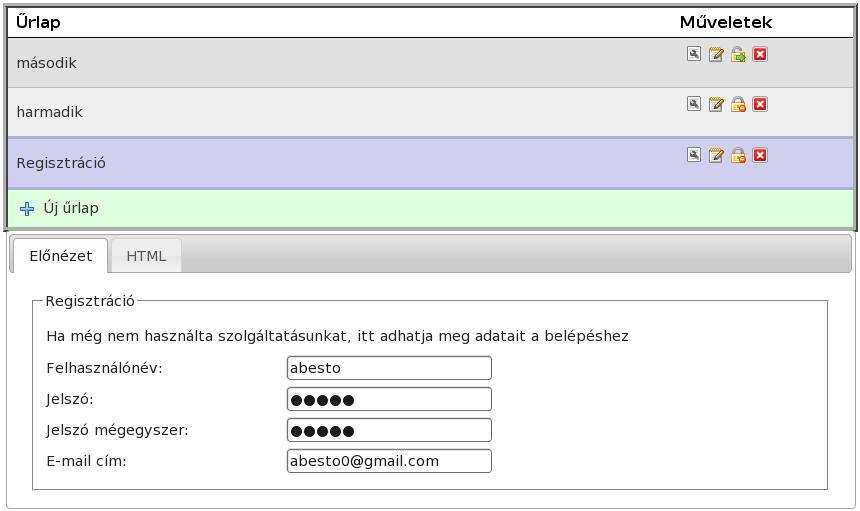
\includegraphics[width=420px]{form_list.png}
  \caption{Űrlapok listája, előnézet}
\end{figure}
\begin{figure}[H]
  
\includegraphics[width=420px]{form_list_html.png}
  \caption{Űrlap HTML nézete}
\end{figure}

Az ``Űrlapjaim'' menüpontból elérhető lista két részből áll: az űrlapokat  és
rajtuk végezhető műveleteket tartalmazó táblázatból, illetve a kiválasztott
űrlap előnézetéből.

\addcontentsline{toc}{section}{Hivatkozások}
\begin{thebibliography}{99}

\bibitem{CI}
  \emph{CodeIgniter framework}\\
  \url{http://codeigniter.com}

\bibitem{CI-ActiveRecord}
  \emph{CodeIgniter felhasználói kézikönyv - Active Record Class}\\
  \url{http://codeigniter.com/user_guide/database/active_record.html}

\bibitem{CI-Req}
  \emph{CodeIgniter felhasználói kézikönyv - Server Requirements}\\
  \url{http://codeigniter.com/user_guide/general/requirements.html}

\bibitem{CI-Val}
  \emph{CodeIgniter felhasználói kézikönyv - Form Validation Class}\\
  \url{http://codeigniter.com/user_guide/libraries/form_validation.html}

\bibitem{CI-Routing}
  \emph{CodeIgniter felhasználói kézikönyv - URI Routing}\\
  \url{http://codeigniter.com/user_guide/general/routing.html}

\bibitem{JQ}
  \emph{jQuery framework}\\
  \url{http://jquery.com}

\bibitem{JQ-LiveQuery}
  \emph{jQuery framework - LiveQuery plugin}\\
  \url{http://jquery.com/Plugins/livequery}

\bibitem{JQ-UI}
  \emph{jQuery framework - user interface}\\
  \url{http://jqueryui.com}

\bibitem{YUI}
  \emph{Yahoo YUI Compressor}\\
  \url{http://developer.yahoo.com/yui/compressor}

\bibitem{MVC}
  \emph{Wikipédia - Modell-nézet-vezérlő}\\
  \url{http://hu.wikipedia.org/wiki/Modell-n\%C3\%A9zet-vez\%C3\%A9rl\%C5\%91}

\bibitem{PHP-SID}
  \emph{PHP kézikönyv - session\_id}\\
  \url{http://hu2.php.net/session_id}

\bibitem{DOM}
  \emph{Wikipedia - Document Object Model}\\
  \url{http://en.wikipedia.org/wiki/Document_Object_Model}

\bibitem{regex}
  \emph{Regular-Expressions.info}\\
  \url{http://www.regular-expressions.info}

\bibitem{ajax}
  \emph{Wikipédia - Ajax (programozás)}\\
  \url{http://hu.wikipedia.org/wiki/Ajax_(programoz\%C3\%A1s)}

\bibitem{json}
  \emph{Wikipedia - JSON}\\
  \url{http://en.wikipedia.org/wiki/Json}

\end{thebibliography}

\end{document}
